\documentclass[10pt]{article}

%------------------------------------------------------
%   PACKAGES
%------------------------------------------------------

% Default 
\usepackage{graphicx}
\usepackage[backend=biber,
  style=numeric, 
  sorting=none]{biblatex}

% Additional
\usepackage{amsmath}
\usepackage{textcomp, gensymb}
\usepackage{placeins}
\usepackage{tabularray} 
\usepackage{xcolor}
\usepackage{placeins}
\usepackage{todonotes}

\newcommand{\td}[1]{\todo[linecolor=blue, backgroundcolor=blue!25,bordercolor=blue, size=\small]{#1}}

\addbibresource{references.bib}

\title{Thin Lens} 
\author{Rahmanyaz Annyyev, Hikmat Gulaliyev}
\date{29 March 2024} 

\begin{document}

\maketitle

\begin{abstract}

\end{abstract}

\section{Introduction}

In the most general sense, a lens is a refracting body that redirects the light rays passing through it. It either focuses or diverges the light rays, depending on the shape of the lens. A simple lens consists of a single piece of transparent material, whereas a compound lens consists of several simple lenses, called elements, usually arranged along a common axis. Lenses are usually made of glass or plastic and are comprised of two surfaces, one or both of which are curved. The most common types of lenses are converging (convex) and diverging (concave) lenses. A converging lens is thicker in the middle than at the edges and focuses light rays to a point called the focal point. A diverging lens is thinner in the middle than at the edges and spreads light rays apart. The focal length of a lens is the distance between the lens and the focal point. The focal length of a converging lens is positive, whereas the focal length of a diverging lens is negative. The thin lens equation relates the object distance, the image distance, and the focal length of a lens. The equation is given by
\begin{equation}
  \frac{1}{f} = \frac{1}{s_{\text{o}}} + \frac{1}{s_{\text{i}}},
\end{equation}
where $f$ is the focal length of the lens, $s_{\text{o}}$ is the object distance, and $s_{\text{i}}$ is the image distance. 

Lenses are divided into two categories: thin lenses and thick lenses. A thin lens is a lens whose thickness is negligible compared to the radii of curvature of the lens surfaces. A thick lens is a lens whose thickness is not negligible compared to the radii of curvature of the lens surfaces. This division depends on a given problem and the accuracy required. 

The experiment is comprised of three parts: A, B, and C. The experimental setup is comprised of a $150$ mm converging lens, a $75$ mm diverging lens, a light source, a crossed arrow target that represents an object, and a screen on which the image is formed. The lenses will be assumed to be thin lenses.

In part A, we will employ the thin lens equation to determine the focal length of the converging lens. The setup is shown in Figure~. First...

\begin{figure}[h]
  \centering
  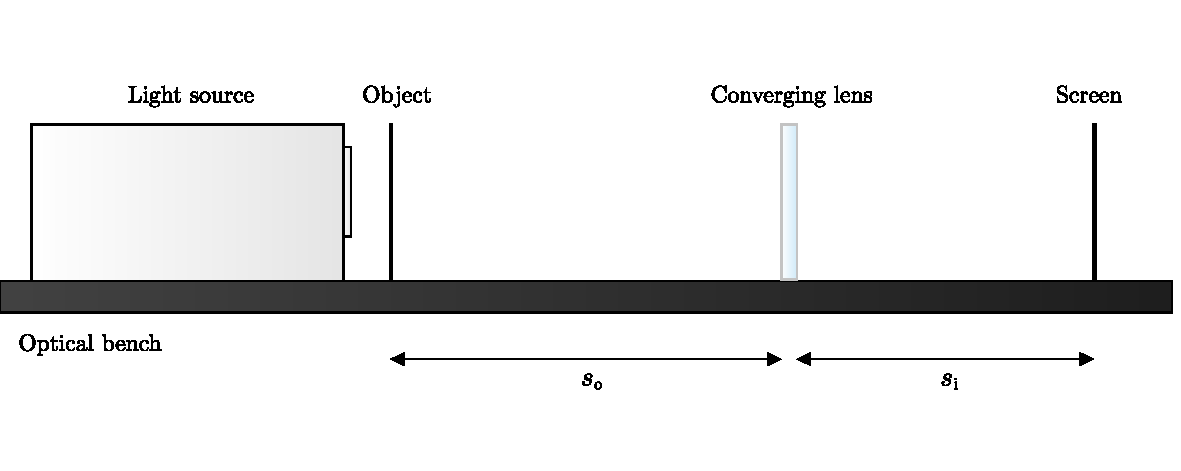
\includegraphics[scale=0.6]{figures/f1.pdf}
  \caption{The experimental setup of part A.}
  \label{fig:1}
\end{figure}

In part B, we will use the Bessel method to determine the focal length of the converging lens. The setup is shown in Figure~. First...

\begin{figure}[h]
  \centering
  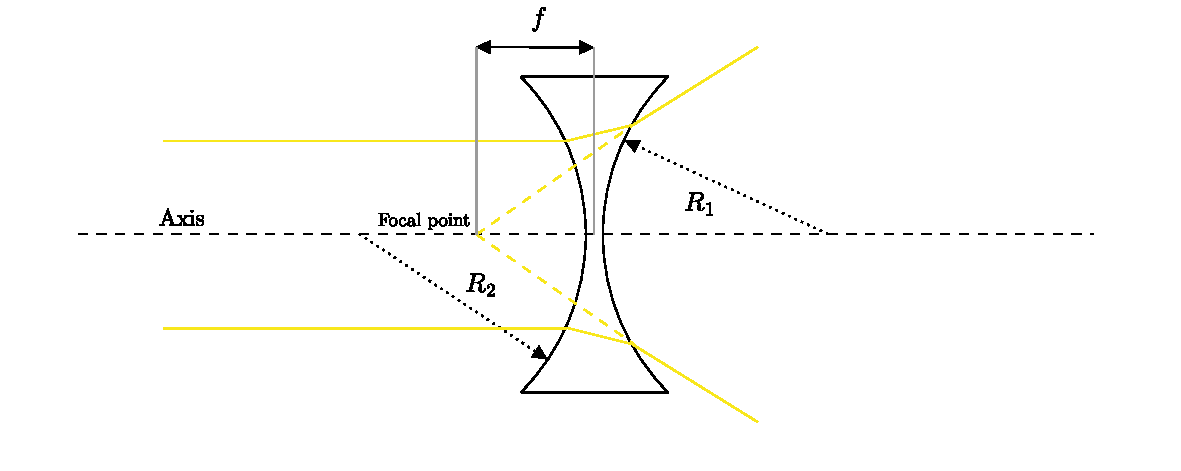
\includegraphics[scale=0.6]{figures/f2.pdf}
  \caption{The experimental setup of part B.}
  \label{fig:2}
\end{figure}

In part C, we will use the virtual object method to determine the focal length of the diverging lens. The setup is shown in Figure~. First...

\begin{figure}[h]
  \centering
  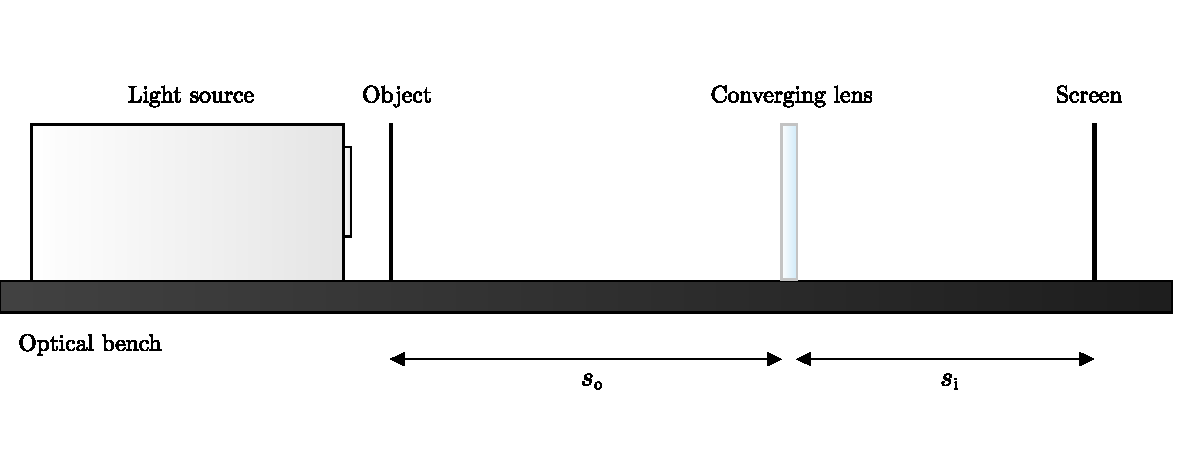
\includegraphics[scale=0.6]{figures/f3.pdf}
  \caption{The experimental setup of part C.}
  \label{fig:3}
\end{figure}

\section{Discussion \& Conclusion}

\section{Data \& Results}

\subsection*{Part A}

The results of part A are shown in Table~\ref{tab:1}. 

\begin{table}[ht]
  \label{tab:1}
  \centering
  \vspace{4mm}
  \begin{tblr}{
    cells = {halign = c, valign = m},
    row{odd} = {bg = lightgray!5},
    row{1} = {bg = lightgray!20},
    hlines = {},
    vlines = {},
    cell{5}{2}={c=2}{c},
    cell{6}{2}={c=2}{c}
  }
    $s_{\text{o}}$ (cm) & $s_\text{{i}}$ (cm) & Focal length, $f_{\text{m}}$ (cm) \\
    \hline
    18 & 12.5 & 7.38 \\
    28 & 10.5 & 7.63 \\
    19.5 & 12.2 & 7.50 \\
    \hline
    Average focal length, $\bar{f}$ (cm) & Error, $\Delta \bar{f}$ (cm) & \\
    7.50 & 0.13 \\ 
  \end{tblr}
  \caption{Results of part A of the experiment.}
\end{table}

\subsection*{Part B}

The results of part B are shown in Table~\ref{tab:2}.

\begin{table}[ht]
  \label{tab:2}
  \centering
  \vspace{4mm}
  \begin{tblr}{
    cells = {halign = c, valign = m},
    row{odd} = {bg = lightgray!5},
    row{1} = {bg = lightgray!20},
    hlines = {},
    vlines = {},
    cell{5}{2}={c=2}{c},
    cell{6}{2}={c=2}{c}
  }
    $d$ (cm) & $D$ (cm) & Focal length, $f_{\text{m}}$ (cm) \\
    \hline
    20.5 & 39.7 & 7.28 \\
    24.5 & 43 & 7.26 \\
    11.2 & 33 & 7.30 \\
    \hline
    Average focal length, $\bar{f}$ (cm) & Error, $\Delta \bar{f}$ (cm) & \\
    7.28 & 0.02 \\ 
  \end{tblr}
  \caption{Results of part B of the experiment.}
\end{table}

\subsection*{Part C}

The results of part C are shown in Table~\ref{tab:3}. The average focal length of the diverging lens is $-15.1$ cm with an error of $0.95$ cm. It is within the limits of error of the actual focal length of the lens, which is $-15$ cm.

\begin{table}[ht]
  \label{tab:3}
  \centering
  \vspace{4mm}
  \begin{tblr}{
    cells = {halign = c, valign = m},
    row{odd} = {bg = lightgray!5},
    row{1} = {bg = lightgray!20},
    hlines = {},
    vlines = {},
    cell{5}{2}={c=3}{c},
    cell{6}{2}={c=3}{c}
  }
    $s_{\text{i}}$ (cm) & $s'_{\text{i}}$ (cm) & d (cm) & Focal length, $f_{\text{m}}$ (cm) \\
    \hline
    16.4 & 22.8 & 7 & -16.0 \\
    18 & 25 & 9 & -14.1 \\
    21 & 46 & 9.6 & -15.2 \\
    \hline
    Average focal length, $\bar{f}$ (cm) & Error, $\Delta \bar{f}$ (cm) & \\
    -15.1 & 0.95 \\ 
  \end{tblr}
  \caption{Results of part C of the experiment.}
\end{table}

\section{Extra credit}

Lenses are a ubiquitous part of our daily lives. They are used in cameras, microscopes, telescopes, and many other devices. In this experiment, we have learned how to determine the focal length of a lens using the thin lens equation, the Bessel method, and the virtual object method. We have also learned how to calculate the magnification of a lens.

\printbibliography

\end{document}